\documentclass[main.tex]{subfiles}
\begin{document}

\subsection{Directory layout}

The project's source code has the following directory structure:
\begin{itemize}
    \item \code{ccg} --- CCGs and CCG parsing
    \item \code{lambda-calculus} --- $\lambda$-terms, type systems, and type-tagging
    \item \code{utils} --- Various utilities
    \item \code{thething} --- Project entry point (CLI interface)
    \item \code{examples}
        \begin{itemize}
            \item \code{library.ccg} --- A library of useful Minipass terms
                (see \cref{stdlib})
            \item \code{amenities.ccg} --- CCG matching rules for the 170 most
                frequently used OpenStreetMap amenities
            \item \code{sample_minipass.ccg} --- a sample Minipass term
            \item \code{sample_grammar.ccg} --- a sample CCG which can parse several
                types of sentences in English
        \end{itemize}
\end{itemize}

\subsection{Running}
The CLI can run in 3 modes:
\begin{itemize}
    \item \emph{summary mode} --- given an input query, generate at most five
        distinct Minipass terms and display them in the terminal along with
        the respective Overpass translations
    \item \emph{\latex mode} --- given an input query, generate a \code{PDF}
        file with at most 10 parses, visualisations of their derivation trees,
        respective Minipass terms and Overpass translations
    \item \emph{web interface mode} --- start a local web server, which provides
        an user interface for entering queries, inspecting the results including
        derivation trees, type hierarchies, and token data, and visualising
        Overpass results on a map via Overpass Turbo\footnote{
            Overpass Turbo is a publicly-available Overpass frontend \cite{overpassturbo}
        }.
\end{itemize}

\greenbox{
    Note: For using the \latex mode and for being to inspect derivation trees
    within the web interface, \code{xelatex} and \code{latexmk} must be installed.
}

For a build system, Haskell's \code{Stack} has been used. The
CLI can be run by issuing:
\begin{lstwrap}\begin{lstlisting}[language=bash]
    $ stack run underpass-exe <arguments>
\end{lstlisting}\end{lstwrap}

When run without arguments, the program loads \code{examples/sample_grammar.ccg}
and starts in web interface mode.

Other modes can be used as follows:
\begin{lstwrap}\begin{lstlisting}[language=bash]
    # Start in web-interface mode and load my_grammar.ccg:
    $ stack run underpass-exe serve my_grammar.ccg

    # Display summary for a given query:
    $ stack run underpass-exe summary my_grammar.ccg 'hospitals in China'

    # Generate a PDF breakdown for a given query:
    $ stack run underpass-exe latex my_grammar.ccg 'hospitals in China'
\end{lstlisting}\end{lstwrap}

\greenbox{
    While the actual running time with the sample grammar is negligible,
    the CLI must load the trained POS tagger and lemmatiser on startup, which
    takes several seconds. Also, drawing trees is relatively slow because it
    uses \latex, so some patience is required.
}

\subsection{Sample results}
These are the contents of \code{examples/sample_grammar.ccg}:
\begin{lstwrap}\begin{lstlisting}
import "library.ccg".
import "amenities.ccg".

begin S.

SE < GSet.

S < GSet.

Entity < GSet.
NamedEntity < String.

mark="begin"  : S / SE        @ \x: SE     => S[GSet[x]] .
mark="end"    : SE \ GSet     @ \x: GSet   => SE[x] .

pos="comma"   : $X \ $X       @ id.

raw="in"
    : GSet / GSet \ GSet
    @ \things, where => and things (in where).

pos="nnp" `'$raw'` : String
    : Entity
    @ name.

pos="nnp" `'$raw'` : String
    : NamedEntity
    @ \x => NamedEntity[x].

raw="like"    : GSet \ NamedEntity @ nameLike.
raw="city"    : GSet \ Entity      @ \x : Entity => and city x.
raw="near"    : GSet \ GSet / GSet @ \b, a => and a (near b).
\end{lstlisting}\end{lstwrap}

We will now, for a more elaborate example, inspect the following query:
\begin{center}
    \code{pharmacies near parking spaces in Berlin}
\end{center}

A relevant excerpt from \code{amenities.ccg} (which defines the phrase
``parking space'') is the following:
\begin{lstwrap}\begin{lstlisting}
lemma="parking" <> lemma="space"
    : Amenity
    @ amenity 'parking_space'.
\end{lstlisting}\end{lstwrap}

So, one\footnote{
    We get two semantic parses for this query: ``pharmacies near parking spaces,
    said pharmacies being in Berlin'' and ``pharmacies near parking spaces,
    said parking spaces being in Berlin''. Both are valid.
} of the derivation trees generated for this query is given below:
\begin{center}
\resizebox{\textwidth}{!}{\begin{tikzpicture}
\Tree [ .{ $S$ } \edge[very thick]; [ .{$($$S$$/_{}$$SE$$)$ } { \minibox[t,frame]{mark:begin}} ]  [ .{ $SE$ }  [ .{ $GSet$ }  [ .{$Amenity$ } { \minibox[t,frame]{pos:nns\\raw:pharmacies\\lemma:pharmacy}} ] \edge[very thick]; [ .{ $($$GSet$$\backslash_{}$$GSet$$)$ } \edge[very thick]; [ .{$($$($$GSet$$\backslash_{}$$GSet$$)$$/_{}$$GSet$$)$ } { \minibox[t,frame]{pos:in\\raw:near\\lemma:near}} ]  [ .{ $GSet$ } \edge[very thick]; [ .{ $($$GSet$$/_{}$$GSet$$)$ }  [ .{ $Amenity$ } \edge[very thick]; [ .{$($$Amenity$$/_{\star}$$Phrase:amenities:54:17$$)$ } { \minibox[t,frame]{pos:nn\\raw:parking\\lemma:parking}} ]  [ .{$Phrase:amenities:54:17$ } { \minibox[t,frame]{pos:nns\\raw:spaces\\lemma:space}} ]  ] \edge[very thick]; [ .{$($$($$GSet$$/_{}$$GSet$$)$$\backslash_{}$$GSet$$)$ } { \minibox[t,frame]{pos:in\\raw:in\\lemma:in}} ]  ]  [ .{$Entity$ } { \minibox[t,frame]{pos:nnp\\raw:Berlin\\lemma:berlin}} ]  ]  ]  ] \edge[very thick]; [ .{$($$SE$$\backslash_{}$$GSet$$)$ } { \minibox[t,frame]{mark:end}} ]  ]  ]
\end{tikzpicture}}
\end{center}

This tree yields the following Minipass term:
\begin{lstwrap}\begin{lstlisting}
symlambda ((symlambda x symabstr S[GSet[x]]) ((symlambda x symabstr SE[x]) ((symlambda b symabstr (symlambda a symabstr ((Amenity  symtot  (GSet  symtot  GSet))[and] a ((symlambda dist symabstr (next (consString 'around' (consNum dist empty)))) 100.0 b)))) ((symlambda things symabstr (symlambda where symabstr ((Amenity  symtot  (GSet  symtot  GSet))[and] things ((List  symtot  (Entity  symtot  GSet))[next] (consString 'in' empty) where)))) ((symlambda _ symabstr ((symlambda k symabstr (symlambda n symabstr ((List  symtot  Amenity)[get] (consString 'tagFilter' (consList (consString '=' (consString k (consString n empty))) empty))))) 'amenity' 'parking_space')) Phrase:amenities:54:17[(symlambda _ symabstr _)]) ((symlambda x symabstr ((GSet  symtot  (GSet  symtot  Entity))[or] (or ((symlambda k symabstr (symlambda n symabstr (get (consString 'tagFilter' (consList (consString '=' (consString k (consString n empty))) empty))))) 'name' x) ((symlambda k symabstr (symlambda n symabstr (get (consString 'tagFilter' (consList (consString '=' (consString k (consString n empty))) empty))))) 'int_name' x)) ((symlambda k symabstr (symlambda n symabstr (get (consString 'tagFilter' (consList (consString '=' (consString k (consString n empty))) empty))))) 'name:en' x))) 'Berlin')) ((symlambda k symabstr (symlambda n symabstr ((List  symtot  Amenity)[get] (consString 'tagFilter' (consList (consString '=' (consString k (consString n empty))) empty))))) 'amenity' 'pharmacy'))))
\end{lstlisting}\end{lstwrap}

Whose types are then squashed:
\begin{lstwrap}\begin{lstlisting}
(( symlambda x symabstr x) (( symlambda x symabstr x) (( symlambda things symabstr ( symlambda where symabstr (and things (next (consString 'in' empty) where)))) (( symlambda b symabstr ( symlambda a symabstr (and a (( symlambda dist symabstr (next (consString 'around' (consNum dist empty)))) 100.0 b)))) (( symlambda _ symabstr (( symlambda k symabstr ( symlambda n symabstr (get (consString 'tagFilter' (consList (consString '=' (consString k (consString n empty))) empty))))) 'amenity' 'parking_space')) ( symlambda _ symabstr _)) (( symlambda k symabstr ( symlambda n symabstr (get (consString 'tagFilter' (consList (consString '=' (consString k (consString n empty))) empty))))) 'amenity' 'pharmacy')) (( symlambda x symabstr (or (or (( symlambda k symabstr ( symlambda n symabstr (get (consString 'tagFilter' (consList (consString '=' (consString k (consString n empty))) empty))))) 'name' x) (( symlambda k symabstr ( symlambda n symabstr (get (consString 'tagFilter' (consList (consString '=' (consString k (consString n empty))) empty))))) 'int_name' x)) (( symlambda k symabstr ( symlambda n symabstr (get (consString 'tagFilter' (consList (consString '=' (consString k (consString n empty))) empty))))) 'name:en' x))) 'Berlin'))))
\end{lstlisting}\end{lstwrap}

And is then $\beta$-reduced:
\begin{lstwrap}\begin{lstlisting}
(and (and (get (consString 'tagFilter' (consList (consString '=' (consString 'amenity' (consString 'pharmacy' empty))) empty))) (next (consString 'around' (consNum 100.0 empty)) (get (consString 'tagFilter' (consList (consString '=' (consString 'amenity' (consString 'parking_space' empty))) empty))))) (next (consString 'in' empty) (or (or (get (consString 'tagFilter' (consList (consString '=' (consString 'name' (consString 'Berlin' empty))) empty))) (get (consString 'tagFilter' (consList (consString '=' (consString 'int_name' (consString 'Berlin' empty))) empty)))) (get (consString 'tagFilter' (consList (consString '=' (consString 'name:en' (consString 'Berlin' empty))) empty))))))
\end{lstlisting}\end{lstwrap}

Finally, after optimisation and translation, we get an Overpass query:
\begin{lstwrap}\begin{lstlisting}
( node["amenity" = "parking_space"]; ) -> .x1;
( area["name" = "Berlin"]; area["int_name" = "Berlin"]; area["name:en" = "Berlin"]; ) -> .x2;
( node(area.x2)(around.x1:100.0)["amenity" = "pharmacy"]; ) -> .x3;
.x3 out;
\end{lstlisting}\end{lstwrap}

When rendering this query with Overpass Turbo, as of the time of writing this
document, we get exactly the result shown in \cref{fig:circles}.
\end{document}
